Consider the three-colorability problem for the following graph:
\begin{figure}[h!]
    \centering
    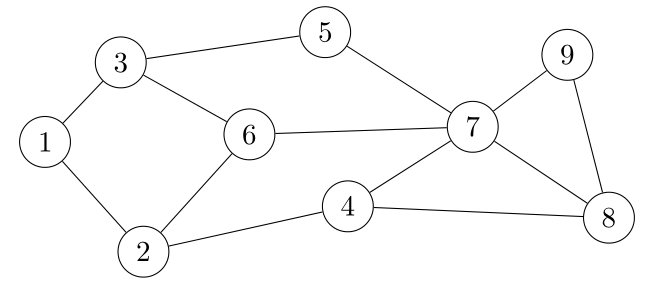
\includegraphics[scale=0.5]{img/cspgraph.png}
\end{figure}

Find a valid 3-coloring for the graph using the colors red, blue, and green. Select the first node by using the \textit{degree heuristic}. After that, select the nodes according to the \textit{minimum remaining values heuristic} and the \textit{degree heuristic} if the remaining values of two or more nodes are equal. If you still have multiple options after applying both heuristics, select the node with the smallest number. Furthermore, select the colors according to the \textit{least constraining value heuristic}.